\documentclass[11pt]{article}
\usepackage[a4paper,margin=2.2cm]{geometry}
\usepackage{amsmath,amssymb,booktabs,graphicx,xcolor,array,multirow,enumitem}
\usepackage[hidelinks]{hyperref}
\graphicspath{{../figures/}{../scratch/interpretation/}}
\definecolor{done}{rgb}{0.1,0.5,0.2}\definecolor{proto}{rgb}{0.75,0.45,0}\definecolor{todo}{rgb}{0.6,0.1,0.1}
\newcommand{\done}{\textcolor{done}{\textbf{done}}}
\newcommand{\proto}{\textcolor{proto}{\textbf{proto}}}
\newcommand{\todo}{\textcolor{todo}{\textbf{todo}}}
\newcommand{\stale}{\textcolor{todo}{\textbf{stale}}}
\newcommand{\GeV}{\,\mathrm{GeV}}
\setlist{itemsep=1pt,topsep=3pt}
\title{Paper 1: claims ledger with current numbers}
\author{Status 14 October 2026 \quad (\texttt{clean} @ \texttt{5e6a42a}, source \texttt{paper/CLAIMS.md})}
\date{}
\begin{document}
\maketitle

\noindent
Paper 1 (Markus's working note): model-independent constraints on the semileptonic gap from the zero-threshold
inclusive moments and the sum-of-exclusives model (SEM). Each claim below is listed with its current numbers and
the pipeline output that produces it. Status: \done{} = pipeline step, reproducible; \proto{} = prototype script,
numbers exist; \stale{} = prototype numbers from the superseded cocktail; \todo{} = not started.

\paragraph{What changed on 14 October.}
The SEM was rebuilt with the Belle~II analysis cocktail and corrected form-factor reweighting (Sec.~\ref{sec:fixes}).
This removes the $M_X^2$ inadmissibility that the September draft and the SLAC seminar reported, and shifts the gap in
$E_\ell$. All numbers in Secs.~\ref{sec:setup}--\ref{sec:data} are from the new cocktail.

\section{Decisions}
\begin{tabular}{@{}p{0.6cm}>{\raggedright\arraybackslash}p{11.2cm}p{3.6cm}@{}}
\toprule
D1 & Primary inclusive input: zero-threshold HQE moments $m_{1..3}$ with likelihood toys (2609.28752) & adopted \\
D2 & Constant $c_\text{true}$ above thresholds dropped; thresholds only via partial BFs (cross-check) & adopted \\
D3 & Polynomial average, per-threshold table, joint fit $\to$ appendix or removed & proposed \\
D4 & MaxEnt densities illustrative; quantitative statements are tests and bounds & adopted \\
D5 & Statements conditional on SEM normalisations; $c_\text{true}\simeq 6$ stated up front & adopted \\
D6 & NR $D^{(*)}\pi\pi\ell\nu$ via $D_1'$/$D_0^*$ (LLSW$\to$BLR, MCAmbulance), split 50:50; PHSP as alternative & adopted 14 Oct \\
D7 & $D$/$D^*$ form factors BLPRXP, one fit, shared eigenvariations & adopted 14 Oct \\
D8 & Candidate $\chi^2$ to Paper 2; Paper 1 keeps kinematic-class support tests & proposed \\
\bottomrule
\end{tabular}

\section{Setup and inputs}\label{sec:setup}

\paragraph{C1 \quad SEM normalisation \hfill \done{} (step 5, \texttt{lib/systematics.py})}
HFLAV branching fractions: $\mathcal{B}_\text{SEM} = 9.26\%$ ($B^+$), $8.55\%$ ($B^0$); gap $1.79\%$ and $1.72\%$,
i.e.\ $\mathcal{B}_\text{gap}/\mathcal{B}_\text{incl} = 0.1647$ (rel.\ unc.\ $15.4\%$), $c_\text{true} = 6.072$.
SEM composition by weight: $D$ $24.6\%$, $D^*$ $57.2\%$, $D^{**}$ $14.8\%$, $D^{(*)}\pi\pi$ $3.1\%$, $D_s^{(*)}K$ $0.3\%$.
All modes normalise to their BF within $1\%$ after weights, except NR $D^{(*)}\pi\pi$ ($0.96$--$0.98$, negligible)
and $D_s^{(*)}K$ ($0.73$/$1.25$, combined spectrum reweight, pre-existing).

\paragraph{C2 \quad Inclusive input \hfill \proto{} (\texttt{measurements\_hqe.py})}
Zero-threshold HQE moments with the full theory covariance; inclusive means and variances:
$\langle M_X^2\rangle = 4.568\GeV^2$, $\mathrm{Var} = 1.618\pm0.083\GeV^4$;
$\langle E_\ell\rangle = 1.390\GeV$, $\mathrm{Var} = 0.185\GeV^2$;
$\langle q^2\rangle = 4.399\GeV^2$, $\mathrm{Var} = 7.935\GeV^4$.

\begin{figure}[h]\centering
\includegraphics[width=0.85\linewidth]{measurements_hqe_3x3.pdf}
\caption{C2: measured moments and the HQE fit as a function of the threshold (independent of the SEM).}
\end{figure}

\paragraph{C3 \quad Inclusive spectrum vs SEM, no subtraction \hfill \done{} (step 8)}
The HQE moments inverted without SEM subtraction are admissible in $100\%$ of the toys for all three observables and need
neither $c_\text{true}$ nor the gap normalisation.

\begin{figure}[h]\centering
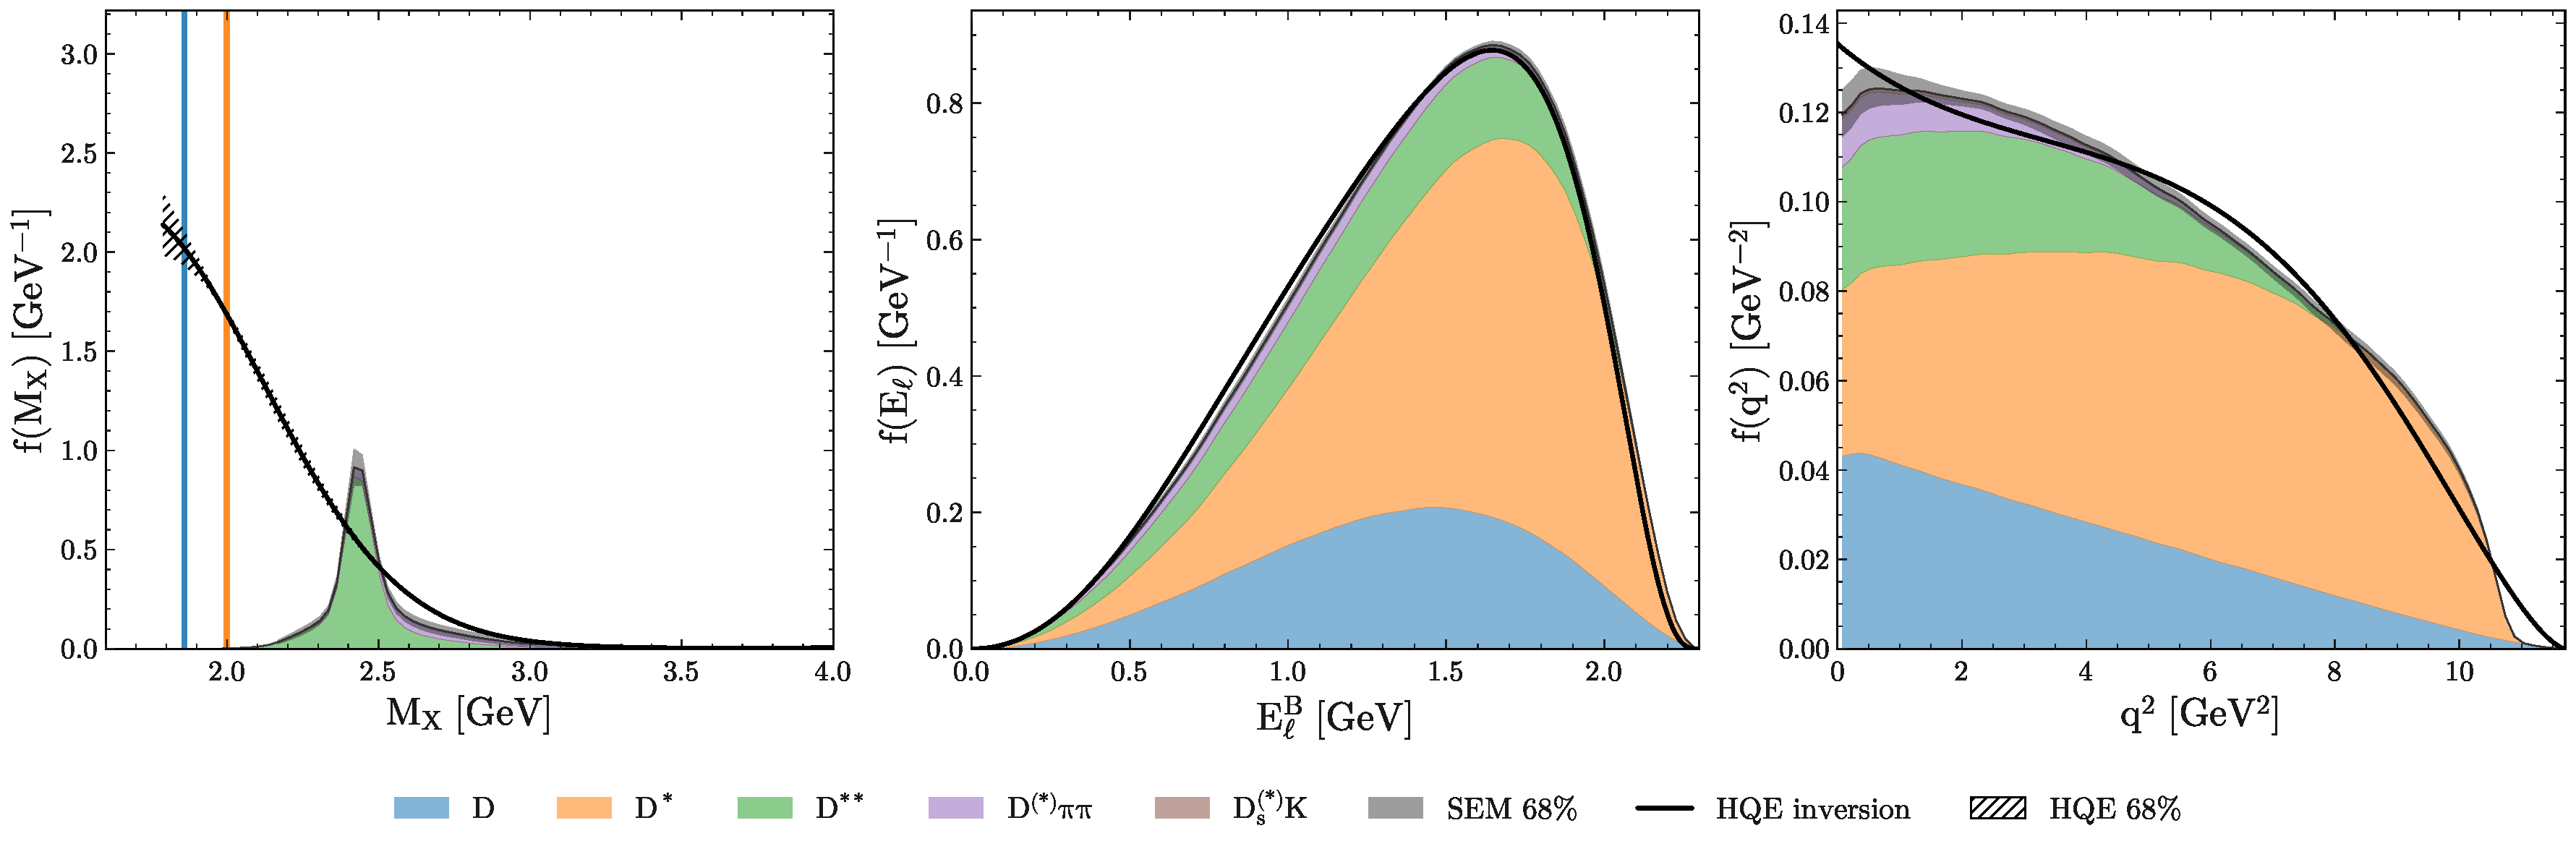
\includegraphics[width=\linewidth]{8/hqe_vs_sem_stack.pdf}
\caption{C3: MaxEnt inversion of the zero-threshold HQE moments (black) against the new SEM, stacked by final state.}
\end{figure}

\section{Validation}

\paragraph{C4 \quad Closure \hfill \done{} (step 7, zero threshold)}
Known gap truths injected into the cocktail and recovered from $m_{1..N}$. Accuracy ($L_1$ distance to the truth) is
unchanged by the new cocktail; admissible fractions for $M_X^2$ improve because the per-mode BF uncertainty is no
longer amplified by the broad PHSP $D^{(*)}\pi\pi$.

\begin{center}\small
\begin{tabular}{llcccc}
\toprule
Truth & Obs. & $N$ & admissible (old $\to$ new) & $L_1$ to truth & \\
\midrule
\multirow{3}{*}{$D_1'\to D^*\eta$} & $M_X^2$ & 3 & $31\% \to 37\%$ & 0.15 & \\
 & $E_\ell$ & 3 & $99\% \to 99\%$ & 0.02 & \\
 & $q^2$ & 3 & $62\% \to 62\%$ & 0.02 & \\
\midrule
\multirow{3}{*}{$50\%\,D\ell\nu + 50\%\,\Lambda_c\bar p\ell\nu$} & $M_X^2$ & 3 / 4 & $59/43\% \to 79/64\%$ & 0.80 / 0.58 & \\
 & $E_\ell$ & 3 & $100\% \to 100\%$ & 0.05 & \\
 & $q^2$ & 3 & $98\% \to 97\%$ & 0.08 & \\
\bottomrule
\end{tabular}
\end{center}
$M_X^2$ remains the weak observable: three moments cannot represent the $D$ line next to a continuum ($L_1 = 1.7$ of a
maximum 2 for $N\le2$).

\begin{figure}[h]\centering
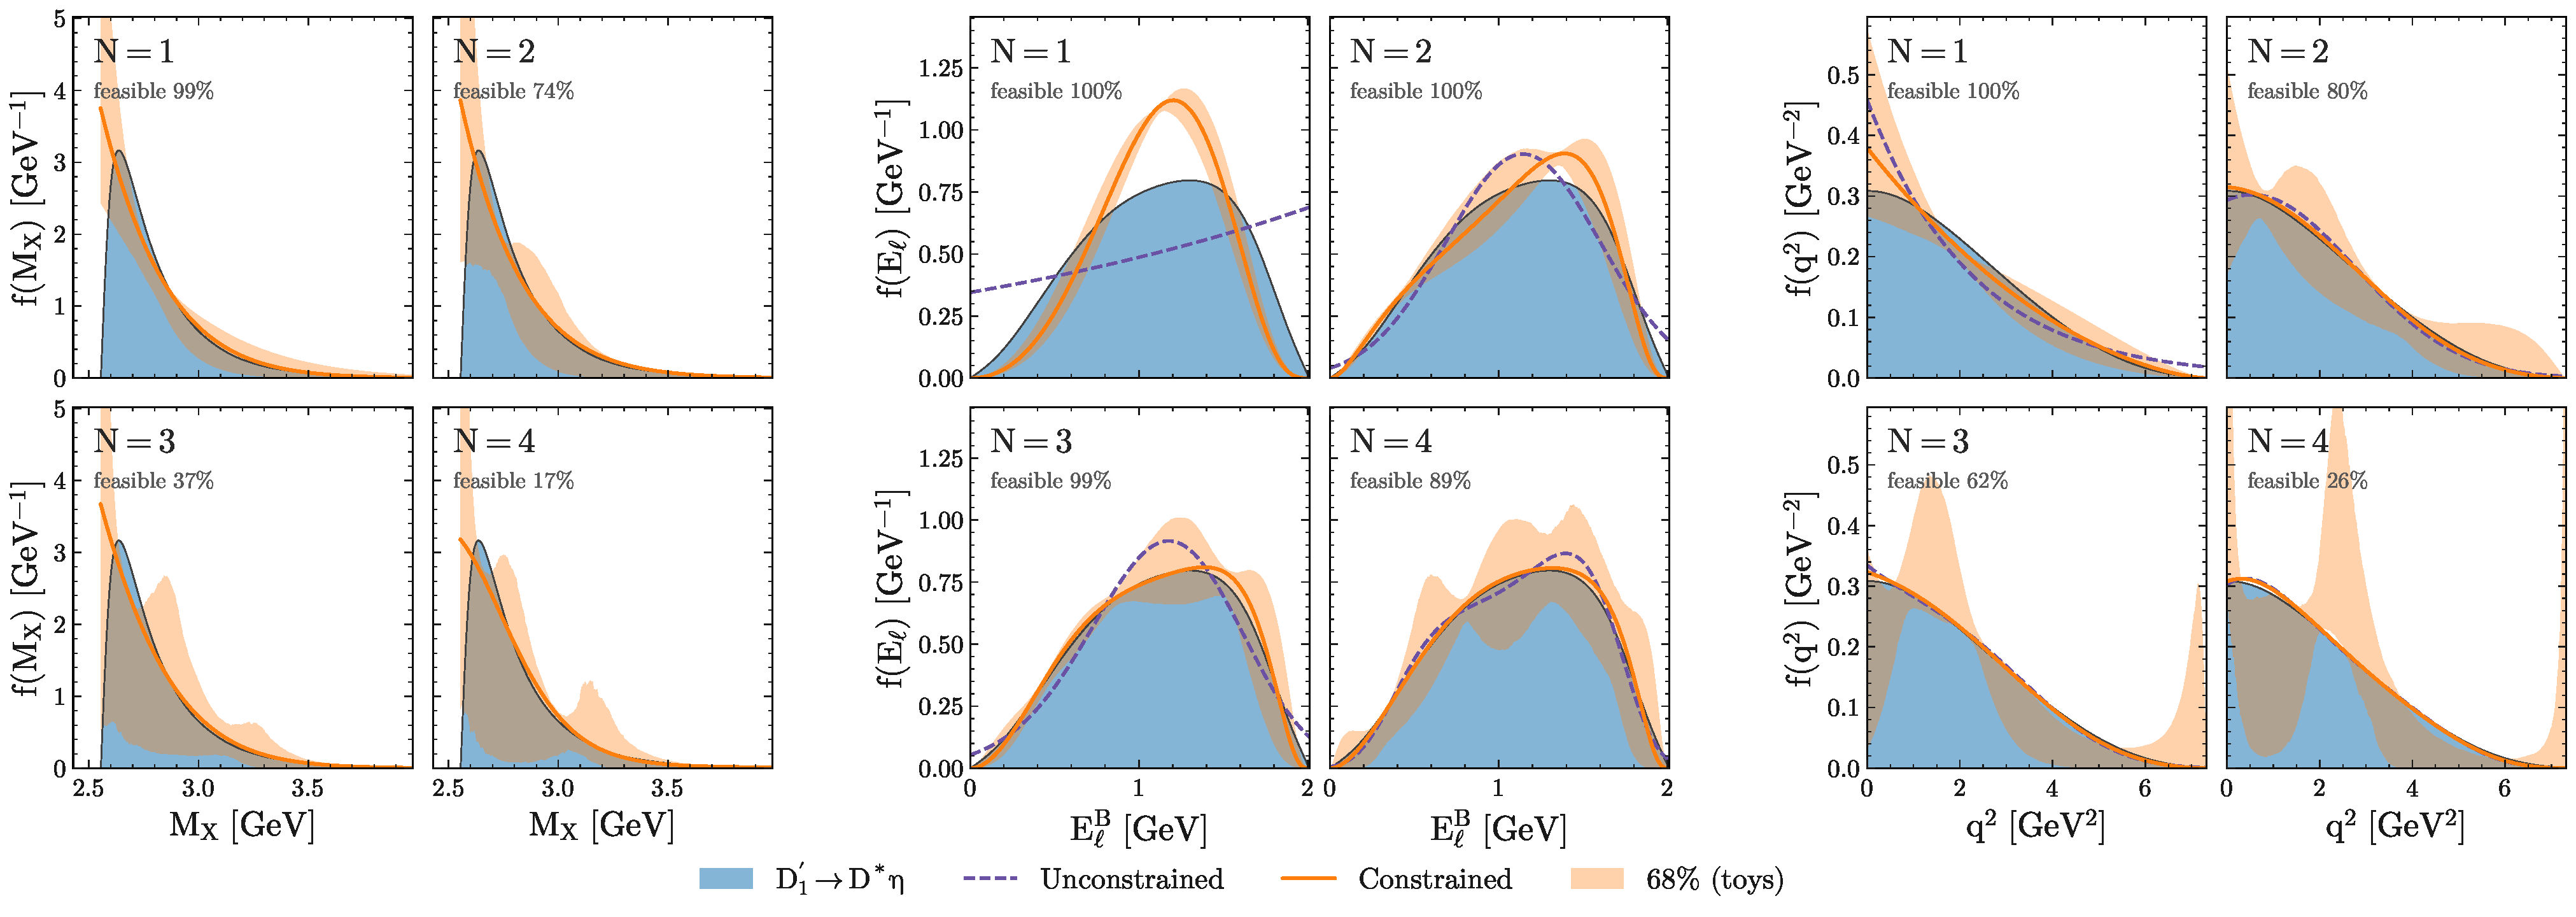
\includegraphics[width=\linewidth]{7/Dp1DstEta/convergence_all3_band.pdf}\\[4pt]
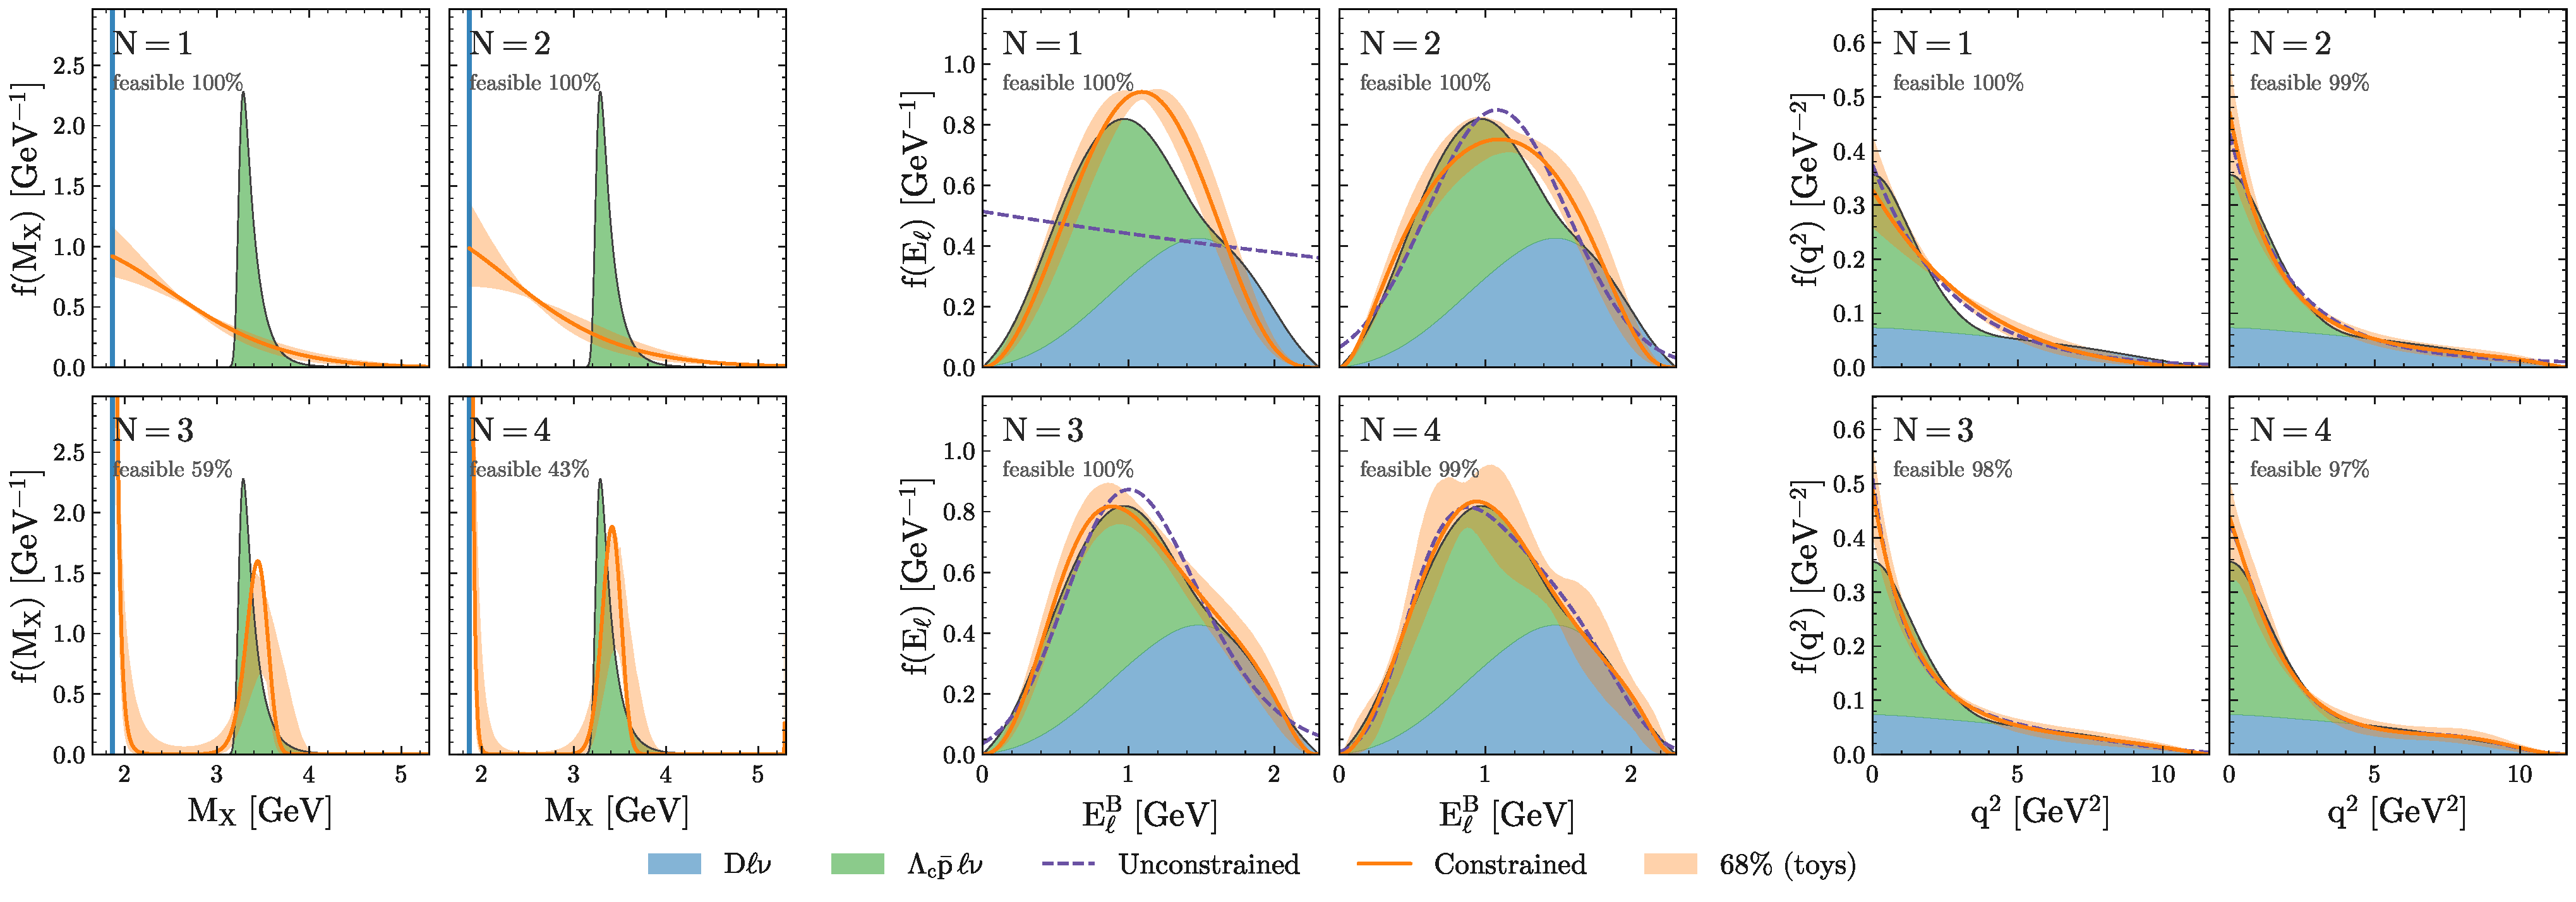
\includegraphics[width=\linewidth]{7/Dlnu_LcPenu/convergence_all3_band.pdf}
\caption{C4: MaxEnt reconstructions for $N=1$--$4$ with $68\%$ bands of the admissible toys; top
$D_1'\to D^*\eta$, bottom the mixed truth.}
\end{figure}

\clearpage
\section{Results on data (zero threshold)}\label{sec:data}

\paragraph{C5 \quad $M_X^2$ is admissible; the PHSP $D^{(*)}\pi\pi$ lineshape is excluded \hfill \done{} (nominal)}
With 5-body PHSP for NR $D^{(*)}\pi\pi\ell\nu$ the SEM was broader than the inclusive spectrum and the residual had
negative variance ($0.4\%$ of toys admissible). With the Belle~II cocktail:

\begin{center}\small
\begin{tabular}{lccc}
\toprule
 & old SEM & new SEM & inclusive (HQE) \\
\midrule
$\mathrm{Var}(M_X^2)$ [GeV$^4$] & 4.06 & \textbf{1.22} & $1.62\pm0.08$ \\
$\langle M_X^2\rangle$ [GeV$^2$] & 4.52 & 4.32 & 4.57 \\
$D^{(*)}\pi\pi$: $\langle M_X^2\rangle$ / Var & 13.8 / 14.8 & 7.5 / 3.5 & \\
$\langle E_\ell\rangle$ [GeV] & 1.394 & 1.408 & 1.390 \\
$\langle q^2\rangle$ [GeV$^2$] & 4.551 & 4.425 & 4.399 \\
$D$: $\langle q^2\rangle$ [GeV$^2$] & 4.09 & 3.67 & \\
\midrule
residual $M_X^2$ admissible (toys) & $0.4\%$ & $\mathbf{75\%}$ & \\
residual $E_\ell$ / $q^2$ admissible & $98\%$ / $99.7\%$ & $100\%$ / $100\%$ & \\
\bottomrule
\end{tabular}
\end{center}
Open: the formal PHSP-vs-resonant comparison (significance with which the moments reject PHSP), part of M2.

\paragraph{C6 \quad Admissibility as a test \hfill \todo{} (M1)}
Current measure is the admissible fraction (above). Replace by a cone-distance statistic with a $p$-value.

\paragraph{C11 \quad Where the gap sits \hfill \proto{} (\texttt{moment\_plane\_clean.py}, rerun 14 Oct)}
Gap mean and variance at zero threshold, $68\%$ toy intervals (HQE $\times$ SEM stat+FF+BF toys), and candidate modes:

\begin{center}\small
\begin{tabular}{lccc}
\toprule
 & $M_X^2$ [GeV$^2$, GeV$^4$] & $E_\ell$ [GeV, GeV$^2$] & $q^2$ [GeV$^2$, GeV$^4$] \\
\midrule
gap mean & $5.83\ [5.36, 6.30]$ & $1.301\ [1.270, 1.334]$ & $4.27\ [4.05, 4.51]$ \\
gap variance & $1.73\ [0.34, 2.43]$ & $0.170\ [0.160, 0.177]$ & $8.01\ [7.42, 8.51]$ \\
$P(\mathrm{Var}<0)$ & $11.5\%$ & 0 & 0 \\
\midrule
$D\pi\pi\pi$ ($D_1$) & 6.05 / 0.83 & 1.330 / 0.169 & 3.18 / 3.63 \\
$D^*\pi\pi\pi$ ($D_2^*$) & 6.32 / 0.75 & 1.159 / 0.165 & 2.81 / 3.25 \\
$D_1'\to D^*\eta$ & 7.88 / 1.97 & 1.120 / 0.172 & 1.97 / 2.00 \\
$D_sK$ & 8.36 / 6.81 & 1.002 / 0.146 & 1.70 / 1.89 \\
$\Lambda_c\bar p$ & 11.46 / 1.24 & 0.826 / 0.091 & 1.04 / 0.62 \\
\bottomrule
\end{tabular}
\end{center}
\begin{itemize}
\item $M_X^2$ and $E_\ell$: $D\pi\pi\pi$ lies at or inside the $68\%$ region.
\item $q^2$: the gap sits on top of the SEM and the inclusive point; every candidate has $\langle q^2\rangle\le3.2\GeV^2$.
  No single candidate explains the gap, and this now rests on $q^2$.
\item Superseded seminar statements: ``gap hard in $E_\ell$'' and ``no low-$E_\ell$ gap'' (the gap density now extends
  to $E_\ell\approx0.3\GeV$, mean $1.30\GeV$ vs $1.37\GeV$ before).
\end{itemize}

\begin{figure}[h]\centering
\includegraphics[width=\linewidth]{moment_plane_clean.pdf}
\caption{C11: mean vs variance of the zero-threshold gap ($68\%$, $95\%$) against the SEM, the inclusive moments and
candidate modes. Grey: no positive density on the data support.}
\end{figure}

\begin{figure}[h]\centering
\includegraphics[width=0.8\linewidth]{gap_density_hqe.pdf}
\caption{C11: MaxEnt inversion of the zero-threshold residual moments ($N=3$, endpoint priors), $68\%$ toy band.
Illustrative only (D4).}
\end{figure}

\paragraph{Uncertainty budget of the zero-threshold residual moments \hfill \done{} (step 8)}
\begin{center}\small
\begin{tabular}{lccc|ccc|ccc}
\toprule
 & \multicolumn{3}{c}{$M_X^2$} & \multicolumn{3}{c}{$E_\ell$} & \multicolumn{3}{c}{$q^2$} \\
Source [\%] & $m_1$ & $m_2$ & $m_3$ & $m_1$ & $m_2$ & $m_3$ & $m_1$ & $m_2$ & $m_3$ \\
\midrule
HQE fit & 2.2 & 3.9 & 5.6 & 0.52 & 1.1 & 1.8 & 1.1 & 2.2 & 3.3 \\
MC stat. & 0.02 & 0.04 & 0.05 & 0.08 & 0.16 & 0.23 & 0.17 & 0.29 & 0.39 \\
Form factors & 5.1 & 11 & 20 & 1.1 & 2.3 & 3.5 & 1.9 & 2.6 & 3.6 \\
$\mathcal{B}$ per mode & 4.1 & 7.9 & 12 & 1.7 & 3.0 & 4.3 & 4.6 & 6.8 & 8.2 \\
$\mathcal{B}_\mathrm{gap}$ & 4.4 & 7.6 & 9.7 & 1.4 & 2.8 & 4.1 & 0.63 & 0.83 & 1.0 \\
\midrule
Total & 8.7 & 18 & 29 & 2.7 & 5.2 & 7.5 & 5.5 & 8.4 & 10 \\
\bottomrule
\end{tabular}
\end{center}
Compared with September, the per-mode BF term for $M_X^2$ dropped from $13/99/99\%$ to $4/8/12\%$; form factors
now dominate $M_X^2$.

\section{Claims not yet supported by current numbers}

\paragraph{C7 \quad Minimal SEM shift \hfill \todo{} (M2)}
Convex fit of BF, $\mathcal{B}_\text{incl}$, FF and lineshape pulls under Hankel positivity of the unnormalised gap
moments. With $M_X^2$ now admissible, the question becomes which pulls the remaining $25\%$ of inadmissible toys and the
$q^2$ tension point to.

\paragraph{C8 \quad Bounds on gap fractions per region \hfill \stale{} (\texttt{interp.py}, old cocktail)}
September prototype (LP, 3 moments): $P(E_\ell\le0.5)\le0.10$, $P(E_\ell\le1.0)\le0.51$, $P(q^2\le6)\ge0.55$.
Must be rerun; the $E_\ell$ bounds in particular will loosen with the softer gap.

\paragraph{C9 \quad Support tests for kinematic classes \hfill \todo{} (M3)}
Endpoints: $\Lambda_c\bar p$ requires $q^2\le4.22\GeV^2$, $E_\ell\le1.66\GeV$; $D_sK$ requires $q^2\le7.94\GeV^2$,
$E_\ell\le2.07\GeV$. Bound the gap mass beyond these, with coverage and a power study (inject $\Lambda_c\bar p$).

\paragraph{C10 \quad Positivity lower-bounds the gap \hfill \stale{}}
September: $E_\ell$, $q^2$ admissible only for $\mathcal{B}_\text{gap}/\mathcal{B}_\text{incl}\gtrsim0.10$--$0.11$. Rerun.

\paragraph{C12 \quad Robustness \hfill \todo{} (M4)}
LHCb cocktail (D** ISGW2 with $D_1'$, $D_0^*$, $D_1$, $D_2^*$; higher $D^{**}$ via $D(2S)$, $D^*(2S)$, $D(2750)$, $D(3000)$;
no NR $D^{(*)}\pi\pi$, no $D_sK$; absolute BFs not in the DecFiles), $\beta=2$ vs $7/2$ for $E_\ell$, support choices,
partial-BF cross-check, PHSP $D^{(*)}\pi\pi$ alternative, $D_1'$:$D_0^*$ split.

\section{Pipeline fixes of 14 October}\label{sec:fixes}
\begin{itemize}
\item Hammer input scheme: the $\tau$ CLN inputs overwrote the light-lepton ones, so all $D$/$D^*$ FF weights were
  target/CLN($\tau$ parameters). Effect at fixed target: $D$ $\le2\%$ per event; $D^*$ $0.54$--$1.83$ per event,
  $q^2$ shape $\pm5\%$, $\langle q^2\rangle$ $+0.08\GeV^2$.
\item $B\to D$ input: EvtGen's BGL has Blaschke factors $=1$ and the \texttt{BGLB2} Hammer class is not in the externals;
  replaced by Hammer-BGL coefficients reproducing EvtGen to $3\times10^{-5}$. $B\to D^*$ input: decfile coefficients.
\item Generation with \texttt{release-09-00-11} (the cocktail's release): $\Gamma(D_1') = 314$ vs $384\,$MeV in 08-02-05,
  as assumed by MCAmbulance.
\item FF slope matrix read only 8 eigenvariations (BLPRXP has 9); streamed step-3 merge; slim step-5 read.
\item KEKCC \texttt{/ghi} tape staging: 38 cocktail and 22 gap-mode samples regenerated instead of recalled.
\end{itemize}

\section{Open inputs}
\begin{tabular}{@{}p{0.6cm}p{11.5cm}>{\raggedright\arraybackslash}p{3.3cm}@{}}
\toprule
I1 & Sign-off on the ledger, D3, D8 & Markus, Danny \\
I2 & BF split of each NR $D^{(*)}\pi\pi$ final state over $D_1'$ and $D_0^*$ (50:50 assumed) & Markus / Philipp \\
I4 & Confirm the HQE toys are the 2609.28752 release; is $m_4$ ($q^2$) available at zero threshold? & Markus \\
I5 & Partial BFs above each $E_\ell$, $q^2$ cut with correlations to the moments & Markus \\
I6 & LHCb cocktail normalisation; higher $D^{**}$ as SEM or gap & note author / Markus \\
I7 & Paper source location and OK to generate figures, tables and numbers into it & Philipp, co-authors \\
\bottomrule
\end{tabular}

\end{document}
